\setcounter{section}{0}
\section{Câu trắc nghiệm nhiều phương án lựa chọn}
\textit{Thí sinh trả lời từ câu 1 đến câu 18. Mỗi câu hỏi thí sinh chọn một phương án}
\setcounter{ex}{0}
\Opensolutionfile{ans}[ans/G12C1TN]
%-------------------------
\begin{ex}
	"Độ không tuyệt đối" là nhiệt độ ứng với
	\choice
	{\True $\SI{0}{\kelvin}$}
	{$\SI{0}{\celsius}$}
	{$\SI{273}{\celsius}$}
	{$\SI{273}{\kelvin}$}
	\loigiai{
	}
	\end{ex}
% ===================================================================
\begin{ex}
\immini{
	Hình bên mô tả chuyển động phân tử ở các thể khác nhau. Hình cầu là phân tử, mũi tên là hướng chuyển động của phân tử. Hình mô tả chuyển động phân tử tương ứng với thể rắn, thể lỏng và thể khí lần lượt là
}
{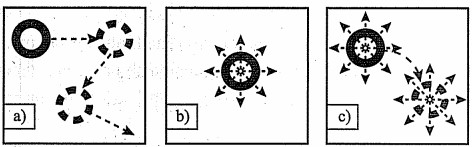
\includegraphics[scale=0.7]{figs/G12-C1-4}
}
\choice
{a), b), c)}
{\True b), c), a)}
{c), b), a)}
{b), a), c)}
	\loigiai{}
\end{ex}
% ===================================================================
\begin{ex}
	Hãy tìm ý \textbf{không đúng} với mô hình động học phân tử.
	\choice
	{Các chất được cấu tạo từ các hạt riêng biệt là phân tử}
	{Các phân tử chuyển động không ngừng}
	{\True Tốc độ chuyển động của các phân tử cấu tạo nên vật càng lớn thì thể tích của vật càng lớn}
	{Giữa các phân tử có lực tương tác gọi là lực liên kết phân tử}
	\loigiai{}
\end{ex}
% ===================================================================
\begin{ex}
	Hãy chọn phương án \textbf{sai} trong các câu sau: Cùng một khối lượng của một chất nhưng khi ở các thể tích khác nhau thì sẽ khác nhau
	\choice
	{thể tích}
	{khối lượng riêng}
	{\True kích thước của các nguyên tử}
	{trật tự của các nguyên tử}
	\loigiai{}
\end{ex}


% ===================================================================
\begin{ex}
Vật ở thể lỏng có	
	\choice
	{thể tích và hình dạng riêng, khó nén}
	{thể tích và hình dạng riêng, dễ nén}
	{\True thể tích riêng nhưng không có hình dạng riêng, khó nén}
	{thể tích riêng nhưng không có hình dạng riêng, dễ nén}
	\loigiai{}
\end{ex}

% ===================================================================
\begin{ex}
	Khi nói đến nhiệt độ của một vật ta thường nghĩ đến cảm giác "nóng" và "lạnh" của vật nhưng đó chỉ là tương đối vì cảm giác mang tính chủ quan. Cảm giác nóng, lạnh mà chúng ta cảm nhận được khi tiếp xúc với vật liên quan đến
	\choice
	{\True năng lượng nhiệt của các phân tử}
	{khối lượng của vật}
	{trọng lượng riêng của vật}
	{động năng chuyển động của vật}
	\loigiai{}
\end{ex}
% ===================================================================
\begin{ex}
	Nội năng của một vật là
	\choice
	{tổng động năng và thế năng của vật}
	{\True tổng động năng và thế năng của các phân tử cấu tạo nên vật}
	{tổng nhiệt lượng và cơ năng mà vật nhận được trong quá trình truyền nhiệt và thực hiện công}
	{nhiệt lượng vật nhận được trong quá trình truyền nhiệt}
	\loigiai{}
\end{ex}
% ===================================================================
\begin{ex}
	Phát biểu nào sau đây là \textbf{đúng}?
	\choice
	{Nội năng của một hệ nhất định phải có thế năng tương tác giữa các hạt cấu tạo nên vật}
	{Nhiệt lượng truyền cho hệ chỉ làm tăng động năng của chuyển động nhiệt của các hạt cấu tạo nên hệ}
	{\True Công mà hệ nhận được có thể làm thay đổi cả tổng động năng chuyển động nhiệt của các hạt cấu tạo nên hệ và thế năng tương tác giữa chúng}
	{Nói chung, nội năng là hàm của nhiệt độ và thể tích, nên nếu thể tích của hệ đã thay đổi thì nội năng của hệ phải thay đổi}
	\loigiai{}
\end{ex}

% ===================================================================
\begin{ex}
	Nhiệt lượng được truyền vào hỗn hợp nước đá để làm tan chảy một phần nước đá. Trong quá trình này, hỗn hợp nước đá
	\choice
	{thực hiện công}
	{có nhiệt độ tăng lên}
	{\True có nội năng tăng lên}
	{thực hiện công, có nhiệt độ tăng và nội năng cũng tăng}
	\loigiai{}
\end{ex}

% ===================================================================
\begin{ex}
	\immini{Hình bên là đồ thị phác hoạ sự thay đổi nhiệt độ theo thời gian trong quá trình chuyển thể từ rắn sang lỏng của chất rắn kết tinh và của chất rắn vô định hình tương ứng lần lượt là
	\choice
	{\True đường (3) và đường (2)}
	{đường (1) và đường (2)}
	{đường (2) và đường (3)}
	{đường (3) và đường (1)}
}{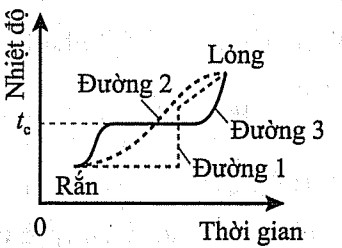
\includegraphics[scale=0.6]{figs/G12-C1-1}}
\loigiai{
\begin{itemize}
	\item Khi nung nóng liên tục một vật rắn kết tinh, nhiệt độ của vật rắn tăng dần. Khi nhiệt độ đạt đến nhiệt độ nóng chảy thì vật bắt đầu chuyển sang thể lỏng và trong suốt quá trình này nhiệt độ của vật không thay đổi. Khi toàn bộ vật rắn đã chuyển sang thể lỏng, nếu tiếp tục cung cấp nhiệt lượng thì nhiệt độ của vật sẽ tiếp tục tăng (đường 3).
	\item Khi nung nóng liên tục vật rắn vô định hình, vật rắn mềm đi và chuyển dần sang thể lỏng một cách liên tục. Trong quá trình này, nhiệt độ của vật tăng lên liên tục. Do đó, vật rắn vô định hình không có nhiệt độ nóng chảy xác định (đường 2).
\end{itemize}
}
	
\end{ex}
% ===================================================================
\begin{ex}
	Gọi $x$, $y$ và $z$ lần lượt là khoảng cách trung bình giữa các phân tử của một chất ở thể rắn, lỏng và khí. Hệ thức đúng là
	\choice
	{$z<y<x$}
	{$x<z<y$}
	{$y<x<z$}
	{\True $x<y<z$}
	\loigiai{}
\end{ex}
% ===================================================================
\begin{ex}
	Một quả bóng có khối lượng $\SI{100}{\gram}$ rơi từ độ cao $\SI{10}{\meter}$ xuống sân và nảy lên được $\SI{7}{\meter}$. Sở dĩ bóng không nảy lên được tới độ cao ban đầu là vì một phần cơ năng của quả bóng đã chuyển hoá thành nội năng của
	\choice
	{chỉ quả bóng và sân}
	{chỉ quả bóng và không khí}
	{chỉ mỗi sân và không khí}
	{\True quả bóng, mặt sân và không khí}
	\loigiai{}
\end{ex}

% ===================================================================
\begin{ex}
	Nếu thực hiện công $\SI{100}{\joule}$ để nén khí trong một xilanh thì khí truyền ra môi trường xung quanh nhiệt lượng $\SI{30}{\joule}$. Xác định độ thay đổi nội năng của khí trong cylanh.
	\choice
	{$\SI{50}{\joule}$}
	{$\SI{60}{\joule}$}
	{$\SI{30}{\joule}$}
	{\True $\SI{70}{\joule}$}
	\loigiai{Hệ nhận công và nhả nhiệt nên: $A=\SI{100}{\joule}$ và $Q=\SI{-30}{\joule}$.\\
		Độ biến thiên nội năng của khí trong xilanh:
		$$\Delta U=A+Q=\SI{70}{\joule}.$$}
\end{ex}
% ===================================================================
\begin{ex}
	Một vật được làm lạnh từ $\SI{25}{\celsius}$ xuống $\SI{5}{\celsius}$. Nhiệt độ của vật theo thang Kelvin giảm đi bao nhiêu Kelvin?
	\choice
	{$\SI{15}{\kelvin}$}
	{\True $\SI{20}{\kelvin}$}
	{$\SI{11}{\kelvin}$}
	{$\SI{18}{\kelvin}$}
	\loigiai{$$\Delta T=\Delta t=\SI{-20}{\kelvin}.$$}
\end{ex}
% ===================================================================
\begin{ex}
Một bình đựng nước ở $\SI{0.00}{\celsius}$. Người ta làm nước trong bình động đặc lại bằng cách hút không khí và hơi nước trong bình ra ngoài. Lấy nhiệt nóng chảy riêng của nước là $\SI{3.3E5}{\joule/\kilogram}$ và nhiệt hoá hơi riêng của nước là $\SI{2.48E6}{\joule/\kilogram}$. Bỏ qua sự trao đổi nhiệt với môi trường bên ngoài. Tỉ số giữa khối lượng nước bị hoá hơi và khối lượng nước ở trong bình lúc đầu là
	\choice
	{\True 0,12}
	{0,84}
	{0,16}
	{0,007}
	\loigiai{Gọi $m$ và $m'$ lần lượt là khối lượng nước ban đầu và khối lượng nước bị hoá hơi. Nhiệt lượng làm hoá hơi hoàn toàn khối lượng nước $m'$ bằng nhiệt lượng làm đông đặc hoàn toàn khối lượng nước $\left(m-m'\right)$.\\
	Ta có:
$$Q_\text{đ}=Q_h\Rightarrow \left(m-m'\right)\lambda=m'L\Rightarrow\dfrac{m'}{m}=\dfrac{\lambda}{\lambda+L}=0,12.$$}
\end{ex}
% ===================================================================
\begin{ex}
	Một học sinh, sau khi biết đến thí nghiệm nổi tiếng của Joule, đã phát triển một thiết bị đạp xe cố định (tập gym), có thể chuyển đổi toàn bộ năng lượng tiêu hao thành nhiệt để làm ấm nước. Cần bao nhiêu cơ năng để tăng nhiệt độ của $\SI{300}{\gram}$ nước $\SI{20}{\celsius}$ đến $\SI{95}{\celsius}$? Biết nhiệt dung riêng của nước là $\SI{4200}{\joule/\left(\kilogram\cdot\kelvin\right)}$.
	\choice
	{\True $\SI{94500}{\joule}$}
	{$\SI{22000}{\joule}$}
	{$\SI{5400}{\joule}$}
	{$\SI{14}{\joule}$}
	\loigiai{
$$Q=mc\Delta T=\SI{94500}{\joule}.$$
}
\end{ex}

% ===================================================================
\begin{ex}
	\immini{Một học sinh dùng một sợi dây buộc vào một vật có khối lượng $\SI{5.0E2}{\kilogram}$ đang rơi qua ròng rọc vào trục bánh guồng. Học sinh này đặt hệ thống vào một bể chứa $\SI{25.0}{\kilogram}$ nước cách nhiệt tốt. Khi vật rơi xuống sẽ làm cho bánh guồng quay và khuấy động nước. Nếu vật rơi một khoảng cách thẳng đứng $\SI{1.00E2}{\meter}$ với vận tốc không đổi thì nhiệt độ của nước tăng bao nhiêu độ? Biết nhiệt dung riêng của nước là $\SI{4.20}{\kilo\joule/\left(\kilogram\cdot\kelvin\right)}$, $g=\SI{9.81}{\meter/\second^2}$.
	\choice
	{$\SI{15}{\kelvin}$}
	{\True $\SI{4.7}{\kelvin}$}
	{$\SI{6.1}{\kelvin}$}
	{$\SI{18}{\kelvin}$}
}
{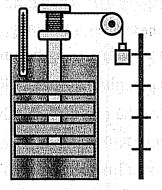
\includegraphics[scale=0.8]{figs/G12-C1-2}}
	\loigiai{Vì vật rơi với vận tốc không đổi nên độ giảm thế năng của nó dùng để làm tăng nhiệt độ cho bình nước.
	$$mgh=m'c\Delta T\Rightarrow \Delta T=\dfrac{mgh}{m'c}=\SI{4.7}{\kilogram}.$$}
\end{ex}
% ===================================================================
\begin{ex}
Một bình cách nhiệt được ngăn làm hai phần bằng một vách ngăn cách nhiệt. Hai phần bình chứa 2 chất lỏng có nhiệt dung riêng $c_1$, $c_2$ và nhiệt độ $t_1$, $t_2$ khác nhau. Bỏ vách ngăn, hai khối chất lỏng không tác dụng hoá học với nhau, nhiệt độ của chất lỏng trong bình sau khi cân bằng nhiệt là $t$. Biết rằng $t_1-t=\dfrac{1}{2}\left(t_1-t_2\right)$. Tỉ số $m_1/m_2$ là	
	\choice
	{$\dfrac{c_1}{c_2}$}
	{\True $\dfrac{c_2}{c_1}$}
	{$\sqrt{\dfrac{c_1}{c_2}}$}
	{$\sqrt{\dfrac{c_2}{c_1}}$}
	\loigiai{
Phương trình cân bằng nhiệt:
\begin{equation}
	m_1c_1\left(t_1-t\right)+m_2c_2\left(t_2-t\right)=0
	\label{eq:C1-5}
\end{equation}	
Theo đề bài, ta có:
$$t_1-t=\dfrac{1}{2}\left(t_1-t_2\right)$$
\begin{equation}
	\Rightarrow t_2-t=t-t_1
	\label{eq:C1-6}
\end{equation}
Thay (\ref{eq:C1-6}) vào (\ref{eq:C1-5}), ta được:
$$m_1c_1\left(t_1-t\right)=m_2c_2\left(t_1-t\right)\Rightarrow \dfrac{m_1}{m_2}=\dfrac{c_2}{c_1}.$$
}
\end{ex}


%-------------------------
\Closesolutionfile{ans}


\section{Câu trắc nghiệm đúng/sai} 
\textit{Thí sinh trả lời từ câu 1 đến câu 4. Trong mỗi ý \textbf{a)}, \textbf{b)}, \textbf{c)}, \textbf{d)} ở mỗi câu, thí sinh chọn đúng hoặc sai}
\setcounter{ex}{0}
\Opensolutionfile{ans}[ans/G12C1TF]
\begin{ex}
	Trong các phát biểu sau đây về sự bay hơi và sự sôi của chất lỏng, phát biểu nào đúng, phát biểu nào sai?
	\choiceTF[t]
	{\True Sự bay hơi là sự hoá hơi xảy ra ở mặt thoáng của khối chất lỏng}
	{\True Sự hoá hơi xảy ra ở cả mặt thoáng và trong lòng của khối chất lỏng khi chất lỏng sôi}
	{Sự bay hơi diễn ra chỉ ở một số nhiệt độ nhất định}
	{\True Sự sôi diễn ra ở nhiệt độ sôi}
	\loigiai{\begin{itemize}
			\item Sự hoá hơi là quá trình chuyển thể từ thể lỏng song thể khí. \item Sự hoá hơi thể hiện qua hai hình thức: sự bay hơi và sự sôi.
			\item Sự sôi xảy ra bên trong và trên bề mặt chất lỏng và chỉ xảy ra ở nhiệt độ sôi.
		\end{itemize}
	}
\end{ex}
% ===============================
\begin{ex}
Hình bên là "giản đồ chuyển thể nhiệt độ/áp suất của nước được đơn giản hoá". Trong các phát biểu sau đây, phát biểu nào đúng, phát biểu nào sai?
\begin{center}
	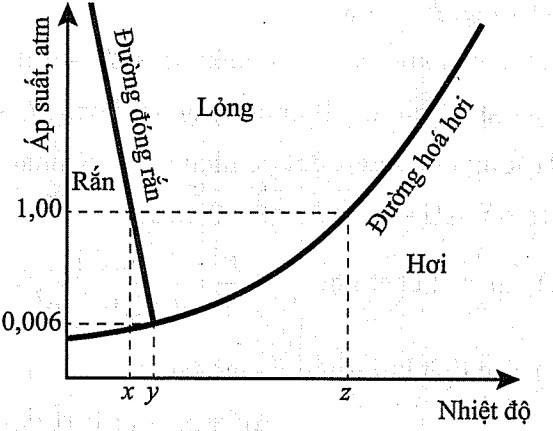
\includegraphics[scale=0.6]{figs/G12-C1-3}
\end{center}
\choiceTF[t]
{\True Thang nhiệt độ Celsius có nhiệt độ dùng làm mốc là nhiệt độ $x$ và nhiệt độ $z$}
{\True Thang nhiệt độ Kelvin có nhiệt độ dùng làm mốc là nhiệt độ thấp nhất mà các vật có thể đạt được (nhiệt độ không tuyệt đối) và nhiệt độ $y$}
{\True Ở nhiệt độ không tuyệt đối, tất cả các chất đều có động năng chuyển động nhiệt của các phân tử bằng không và thế năng của chúng là tối thiểu}
{Hiện nay, các nhà khoa học đã hạ thấp nhiệt độ đến $\SI{0}{\kelvin}$}	


	
	\loigiai{Thang nhiệt độ Celsius có nhiệt độ dùng làm mốc là nhiệt độ tan chảy của nước tinh khiết khi đóng băng và nhiệt độ sôi của nước tinh khiết ở áp suất tiêu chuẩn.\\
	Thang nhiệt độ Kelvin có nhiệt độ dùng làm mốc là nhiệt độ thấp nhất mà các vật có thể đạt được (nhiệt độ không tuyệt đối) và nhiệt độ mà nước tinh khiết có thể tồn tại đồng thời cả ba thể rắn, lỏng và hơi.\\
	Ở nhiệt độ không tuyệt đối, tất cả các chất đều có động năng chuyển động nhiệt của các phân tử bằng không và thế năng của chúng là tối thiểu.\\
	Vật lí học hiện đại chứng tỏ, các hạt không thể đứng yên, điều này có nghĩa chỉ có thể hạ nhiệt độ xuống gần giá trị $\SI{0}{\kelvin}$ nhưng không thể đạt đến giá trị này. Hiện nay, nhiệt độ thấp nhất mà các nhà khoa học có thể tạo ra là $\SI{3.8E-11}{\kelvin}$.
	}
\end{ex}
% ===============================
\begin{ex}
	Nhiệt nóng chảy riêng và nhiệt độ nóng chảy là thông tin, giúp ta có thể
	\choiceTF[t]
	{\True xác định được năng lượng cần cung cấp cho lò nung, thời gian nung}
	{\True thời điểm đổ kim loại nóng chảy vào khuôn, thời điểm lấy sản phẩm ra khỏi khuôn}
	{\True lựa chọn vật liệu chế tạo hợp kim phù hợp với từng yêu cầu sử dụng khác nhau}
	{\True tách các kim loại nguyên chất ra khỏi quặng hỗn hợp}	
	
	\loigiai{}
\end{ex}
% ===============================
\begin{ex}
Một bình đun nước nóng bằng điện có công suất $\SI{9.0}{\kilo\watt}$. Nước được làm nóng khi đi qua buồng đốt của bình. Nước chảy qua buồng đốt với lưu lượng $\SI{5.8E-2}{\kilogram/\second}$. Nhiệt độ của nước khi đi vào buồng đốt là $\SI{15}{\celsius}$. Cho nhiệt dung riêng của nước là $\SI{4200}{\joule/\left(\kilogram\cdot\kelvin\right)}$. Bỏ qua mọi hao phí.
	\choiceTF[t]
	{Nhiệt độ của nước khi ra khỏi buồng đốt là $\SI{50}{\celsius}$}
	{Nếu nhiệt độ của nước khi đi vào buồng đốt tăng gấp đôi thì nhiệt độ nước ra khỏi buồng đốt tăng gấp đôi}
	{\True Nếu công suất điện giảm 2 lần thì nhiệt độ nước ra khỏi buồng đốt là $\SI{33.5}{\celsius}$}
	{\True Để điều chỉnh nhiệt độ của nước ra khỏi buồng đốt, ta có thể thay đổi: công suất điện; lưu lượng nước; nhiệt độ nước đi vào}	

	\loigiai{\begin{itemchoice}
			\itemch Gọi $q$ là lưu lượng nước chảy vào buồng đốt và $\calP$ là công suất buồng đốt.\\
			Nhiệt độ của nước khi ra khỏi buồng đốt:
			$$qtc\left(t_2-t_1\right)=\calP t\Rightarrow t_2=t_1+\dfrac{\calP}{qc}\approx\SI{51.9}{\celsius}.$$
			\itemch Sai vì $t_2=t_1+\dfrac{\calP}{qc}$.
			\itemch Đúng. 
			$$t'_2=t_1+\dfrac{\calP}{2qc}=\SI{33.5}{\celsius}.$$
			\itemch Đúng. $t_2$ phụ thuộc vào $\calP$, $q$ và $t_1$.
			\end{itemchoice}
	}
\end{ex}
\Closesolutionfile{ans}
\section{Câu trắc nghiệm trả lời ngắn} \textit{Thí sinh trả lời từ câu 1 đến câu 6}
\setcounter{ex}{0}
\Opensolutionfile{ans}[ans/G12C1TL]
% ===============================================================
\begin{ex}
	Một người cọ xát một miếng sắt có khối lượng $\SI{0.25}{\kilogram}$ trên một sàn nhà. Sau một thời gian miếng sắt nóng thêm $\SI{12.0}{\celsius}$. Tính công mà người này đã thực hiện \textit{(theo đơn vị $\si{\joule}$, lấy phần nguyên)}. Giả sử rằng $\SI{40}{\percent}$ công đó được dùng làm nóng miếng sắt. Biết nhiệt dung riêng của sắt là $\SI{0.46}{\kilo\joule/\left(\kilogram\cdot\kelvin\right)}$.
	\shortans{$\SI{3450}{}$}
	\loigiai{
		$$0,4A=mc\Delta T\Rightarrow A=\SI{3450}{\joule}.$$
	}
\end{ex}
% ===============================================================
\begin{ex}
	Một viên đạn chì phải có tốc độ tối thiểu là bao nhiêu để khi nó va chạm vào vật cản cứng thì nóng chảy hoàn toàn \textit{(theo đơn vị $\si{\meter/\second}$, lấy phần nguyên)}? Cho rằng $\SI{80.0}{\percent}$ động năng của viên đạn chuyển thành nội năng của nó khi va chạm; Nhiệt độ của viên đạn trước khi và chạm là $\SI{127}{\celsius}$. Cho biết nhiệt dung riêng của chì là $c=\SI{0.130}{\kilo\joule/\left(\kilogram\cdot\kelvin\right)}$; nhiệt độ nóng chảy của chì là $\SI{327}{\celsius}$, nhiệt nóng chảy riêng của chì là $\lambda=\SI{25.0}{\kilo\joule/\kilogram}$.
	\shortans{357}
	\loigiai{
		$$\SI{80}{\percent}\cdot\dfrac{1}{2}mv^2=mc\Delta T+m\lambda\Rightarrow v=\sqrt{\dfrac{2\left(c\Delta T+\lambda\right)}{0,8}}\approx\SI{357}{\meter/\second}.$$
	}
	\end{ex}
	% ===============================================================
\begin{ex}
	Một vật có khối lượng $\SI{1.00}{\kilogram}$ trượt trên một mặt phẳng nghiêng dài $\SI{0.800}{\meter}$ đặt nghiêng $\SI{30.0}{\degree}$. Ở đỉnh của mặt phẳng nghiêng, vận tốc của vật bằng 0; trượt tới chân mặt phẳng nghiêng, tốc độ của vật đạt $\SI{1.10}{\meter/\second}$. Lấy $g=\SI{9.81}{\meter/\second^2}$. Tính nhiệt lượng do vật toả ra do ma sát \textit{(theo đơn vị $\si{\joule}$, lấy đến hai chữ số ở phần thập phân)}.
	\shortans{3,32}
	\loigiai{
		Nhiệt lượng tăng thêm bằng độ lớn công của lực cản và bằng độ giảm cơ năng:
		$$Q=mgh-\dfrac{1}{2}mv^2=mgL\sin\SI{30.0}{\degree}-\dfrac{1}{2}mv^2=\SI{3.32}{\joule}.$$
	}
\end{ex}
	% ===============================================================
\begin{ex}
Ở nhiệt độ $\SI{27}{\celsius}$, các phân tử oxygen chuyển động với tốc độ trung bình khoảng $\SI{500}{\meter/\second}$. Khối lượng của phân tử oxygen là $\SI{53.2E-27}{\kilogram}$. Động năng trung bình của $\SI{E21}{}$ phân tử oxygen bằng bao nhiêu \textit{(viết đáp số 3 kí tự số)}?
	\shortans{6,65}
	\loigiai{
	$$W_\text{đ}=\dfrac{1}{2}Nmv^2=\SI{6.65}{\joule}.$$
	}
\end{ex}
	% ===============================================================
\begin{ex}
Nhiệt lượng kế bằng đồng chứa nước ở $\SI{25}{\celsius}$. Khối lượng tổng cộng của nhiệt lượng kế là $\SI{475}{\gram}$. Bỏ vào nhiệt lượng kế một vật bằng đồng có nhiệt dung riêng $c_3=\SI{0.08}{cal/\left(\gram\cdot\kelvin\right)}$, khối lượng $\SI{400}{\gram}$ ở $\SI{90}{\celsius}$. Nhiệt độ sau cùng của hệ khi cân bằng nhiệt là $\SI{30}{\celsius}$. Tính khối lượng của nhiệt lượng kế theo đơn vị gram. Biết nhiệt dung riêng của nhiệt lượng kế và nước lần lượt là $c_1=\SI{0.09}{cal/\left(\gram\cdot\kelvin\right)}$; $c_2=\SI{1}{cal/\gram\cdot\kelvin}$.
	\shortans{100}
	\loigiai{
	Áp dụng phương trình cân bằng nhiệt:
	$$Q_1+Q_2+Q_3=0$$
	\begin{equation}
		\Rightarrow 0,45m_1+5m_2=1920
		\label{eq:C1-1}
	\end{equation}
Mặt khác:
\begin{equation}
	m_1+m_2=\SI{475}{\gram}
	\label{eq:C1-2}
\end{equation}
Từ (\ref{eq:C1-1}) và (\ref{eq:C1-2}), thu được: $m_1=\SI{100}{\gram}.$
	}
\end{ex}
	% ===============================================================
\begin{ex}
	Lấy $\SI{0.01}{\kilogram}$ hơi nước ở $\SI{100}{\celsius}$ cho ngưng tụ trong bình nhiệt lượng kế chứa $\SI{0.25}{\kilogram}$ nước ở $\SI{10}{\celsius}$; nhiệt độ cuối cùng là $\SI{35}{\celsius}$. Cho nhiệt dung riêng của nước là $c=\SI{4180}{\joule/\left(\kilogram\cdot\kelvin\right)}$. Nhiệt hoá hơi riêng của nước bằng bao nhiêu \textit{(tính theo đơn vị $\SI{E6}{\joule/\kilogram}$, làm tròn đến 2 chữ số thập phân)}.
	\shortans{2,34}
	\loigiai{
		Áp dụng phương trình cân bằng nhiệt:
		$$-m_\text{h}L-m_\text{h}c\left(t_\text{cb}-100\right)+m_\text{n}c\left(t_\text{cb}-t_0\right)=0\Rightarrow L\approx\SI{2.34E6}{\joule/\kilogram}.$$
	}
\end{ex}
\Closesolutionfile{ans}
\begin{center}
	\textbf{--- HẾT ---}
\end{center}